\documentclass{article}
\usepackage{graphicx}
\usepackage{float}
\usepackage{subcaption}
\usepackage{listings}
\usepackage{amsmath}
\usepackage{amsfonts}
\usepackage[square, numbers]{natbib}
\bibliographystyle{unsrtnat}
\usepackage[colorlinks=true, allcolors=blue]{hyperref}
\usepackage{xcolor}

\definecolor{mGreen}{rgb}{0,0.6,0}
\definecolor{mGray}{rgb}{0.5,0.5,0.5}
\definecolor{mPurple}{rgb}{0.58,0,0.82}
\definecolor{backgroundColour}{rgb}{0.95,0.95,0.92}

\lstdefinestyle{CStyle}{
    backgroundcolor=\color{backgroundColour},   
    commentstyle=\color{mGreen},
    keywordstyle=\color{magenta},
    numberstyle=\tiny\color{mGray},
    stringstyle=\color{mPurple},
    basicstyle=\footnotesize,
    breakatwhitespace=false,         
    breaklines=true,                 
    captionpos=b,                    
    keepspaces=true,                 
    numbers=left,                    
    numbersep=5pt,                  
    showspaces=false,                
    showstringspaces=false,
    showtabs=false,                  
    tabsize=2,
    language=C
}
\bibliographystyle{alpha}

\title{Information Theory \\ \large Problem Set 09 - Decision Theory}
\author{Luís Felipe Ramos Ferreira}
\date{\href{mailto:lframos\_ferreira@outlook.com}{\texttt{lframos\_ferreira@outlook.com}}
}

\begin{document}

\maketitle

\begin{enumerate}
	\item \begin{enumerate}
		      \item The set of all states the world or reality can be at.
		      \item The set of actions an entity can take in the world.
		      \item It's a function that measures the benefits of and entity taking an action \(a\) if the current state of the world is \(s\). If the benefits of taking the action \(a\) in state \(s\) is high, then the value of the utility function
		            with the pair \((a, s)\) is also high.
		      \item We are trying to maximize the expected value of the utility function if we take the action \(a\) in the current state. In formal therms, we want to find the action \(a\) that maximizes
		            \[E(U | a) = \sum_x p(x | a)u(a, x)\],
		            where \(a(u, x)\) is the utility function when we take action \(a\) in the state \(x\).
	      \end{enumerate}
	\item Question answered by hand.
	      \begin{figure}[H]
		      \centering
		      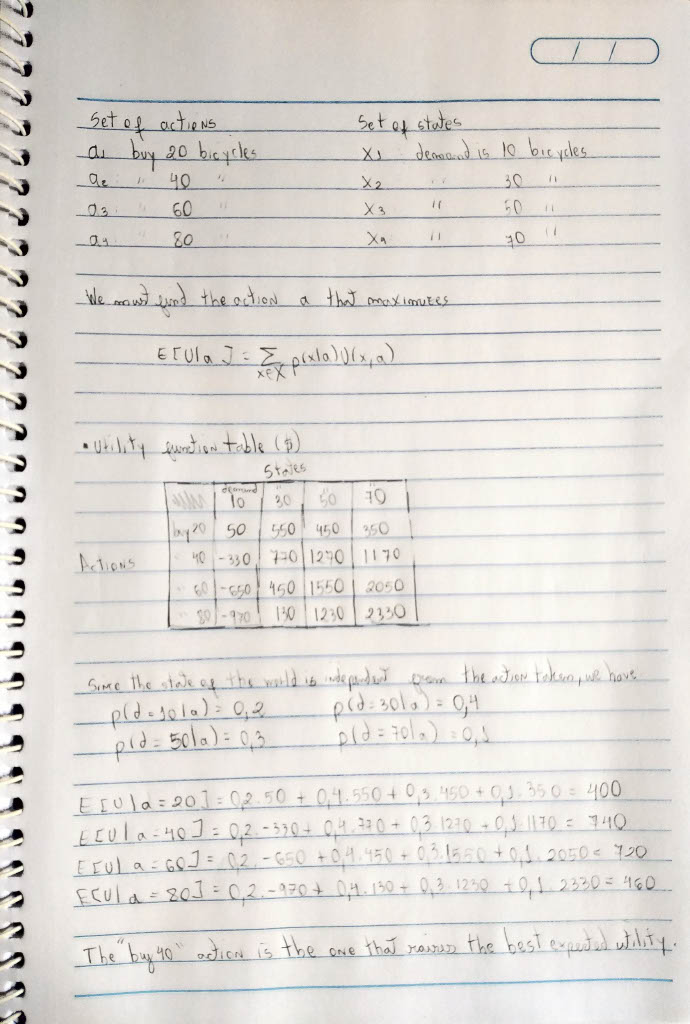
\includegraphics[width=0.5\textwidth]{images/02.jpeg}
		      \caption{Problem 02}
	      \end{figure}
	\item The set of states are \(\{0, 1, 2.5\}\), the possible amounts of million pounds that a person can gain in the world.
	      The set of actions is \(\{A, B, C, D\}\). Usually the utility function \(u: \mathcal{A} \times \mathcal{X} \rightarrow \mathbb{R}\)
	      is a function of a pair of action and current state of the world to some real value. In this case the utility function depends only in the current state of the world,
	      so we can say the utility function is \(u: \mathcal{X} \rightarrow \mathbb{R}\).

	      The utility function table is given by the following table:

	      \bigskip
	      \begin{center}
		      \begin{tabular}{|c|c|c|c|}
			      \hline
			      X & 0    & 1    & 2.5  \\ \hline
			      A & 0    & 1    & 0    \\ \hline
			      B & 0.01 & 0.89 & 0.1  \\ \hline
			      C & 0.89 & 0.11 & 0    \\ \hline
			      D & 0.90 & 0.0  & 0.10 \\ \hline
		      \end{tabular}
	      \end{center}

	      We must now calculate the expected utility of each action and infer a absurd to prove the choices of the entities in this game makes no sense
	      and that humans in general see the expected utility of money in a weird way.

	      \begin{figure}[H]
		      \centering
		      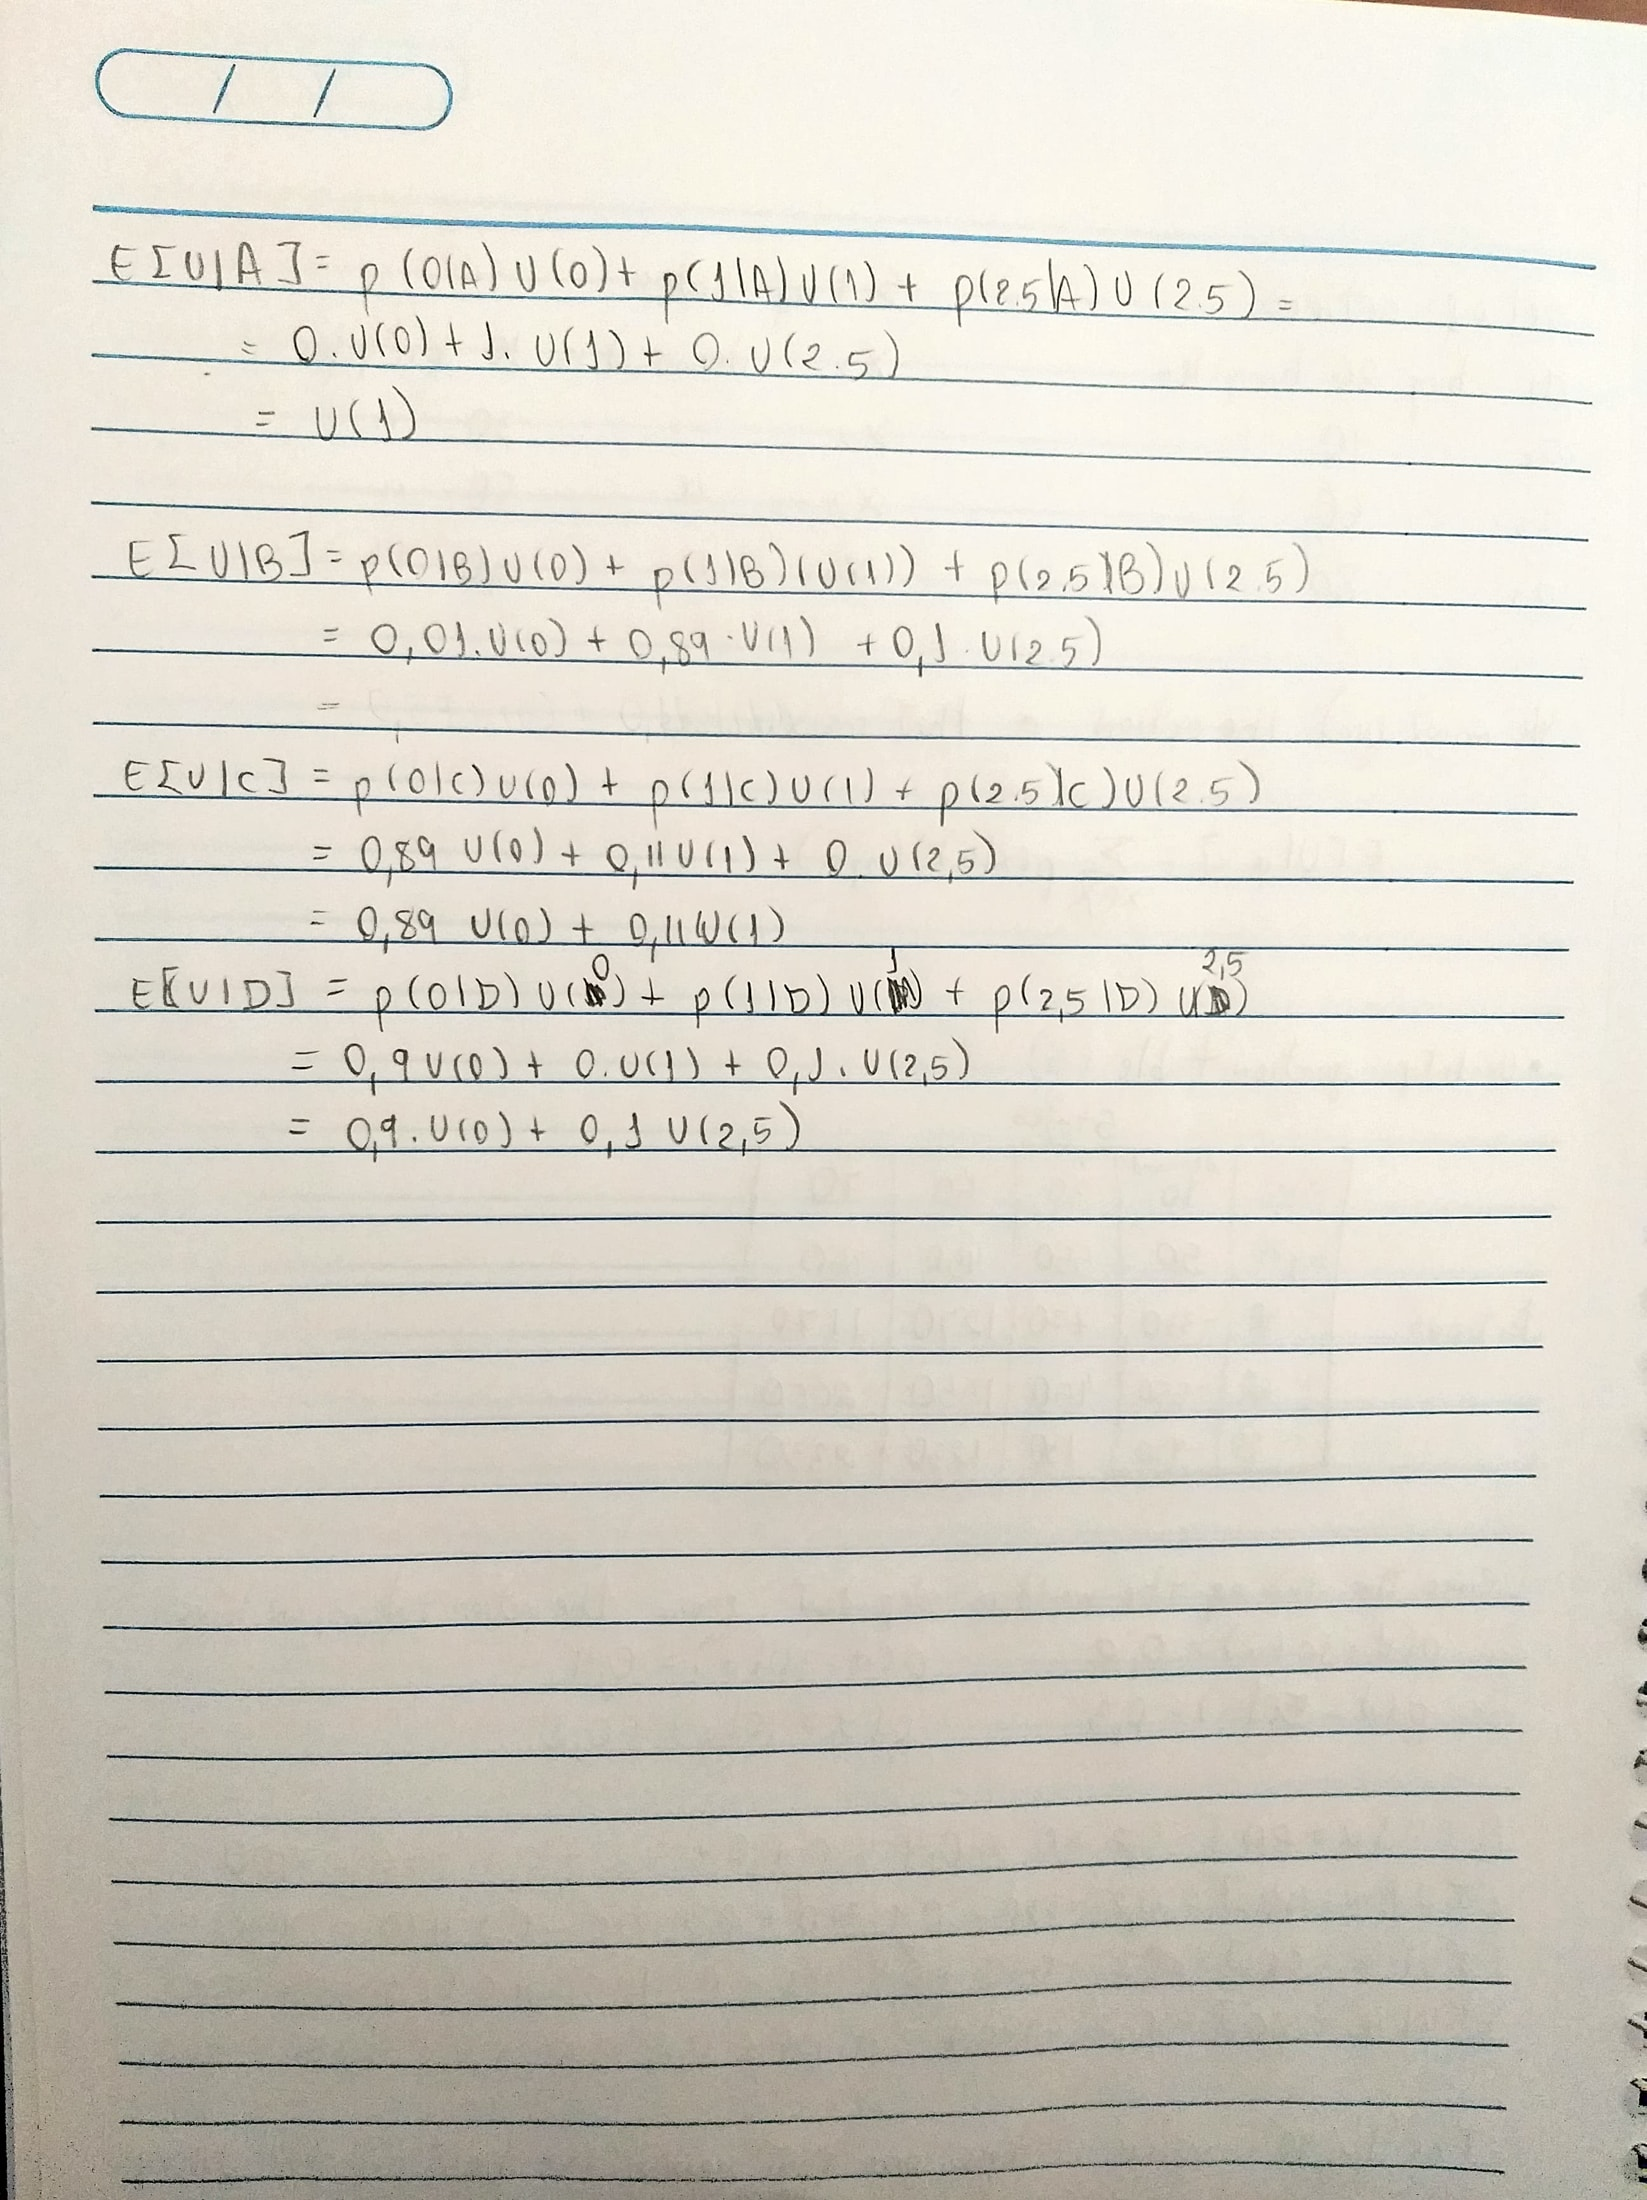
\includegraphics[width=0.5\textwidth]{images/03.jpeg}
		      \caption{Problem 03 calculations}
	      \end{figure}

	      \[E[U \mid A] = U(1)\]
	      \[E[U \mid B] = 0.01*U(0) + 0.89*U(1) + 0.10*U(2.5)\]
	      \[E[U \mid C] = 0.89*U(0) + 0.11*U(1)\]
	      \[E[U \mid D] = 0.9*U(0) * 0.10*U(2.5)\]

	      But, if the choices from the entities is \(A\) over \(B\) and \(D\) over \(C\), we have:

	      \[U(1) > 0.01*U(0) + 0.89*U(1) + 0.10*U(2.5)\]
	      \[U(0) - 11*U(1) + 10*U(2.5) < 0\]

	      and,

	      \[0.9*U(0) * 0.10*U(2.5) < 0.89*U(0) + 0.11*U(1)\]
	      \[U(0) - 11*U(1) + 10*U(2.5) > 0\]

	      which is clearly an absurd.
\end{enumerate}

\bibliography{sample}
\nocite{*}

\end{document}
